% !TEX root = main.tex

\section{空间域图像增强} % Chap 3
图像增强目的是提高图像在特定应用领域的视觉质量,包括光滑、锐化、提取边缘、反转、去噪以及各种滤波等。

空间域图像增强的是直接对图像的像素进行操作,基本关系式可表示如下:
\[g(x,y)=T(f(x,y))\]

\subsection{基本灰度变换}
\begin{itemize}
\item 基本灰度函数:线性、对数、幂次
\begin{figure}[H]
\centering
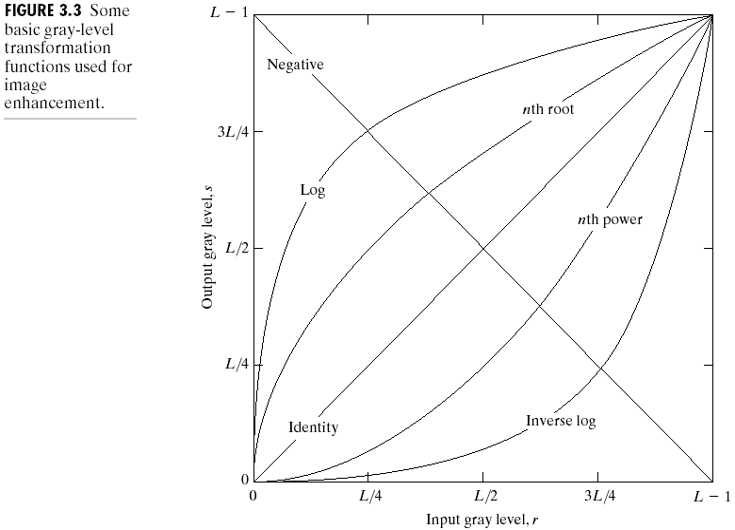
\includegraphics[width=0.6\linewidth]{fig/enhancement.png}
\end{figure}
\item 图像反转变换:$s=L-1-r$,人眼的一个特点就是在背景相对光亮时对灰度层次有较好的分辨能力。
\begin{figure}[H]
\centering
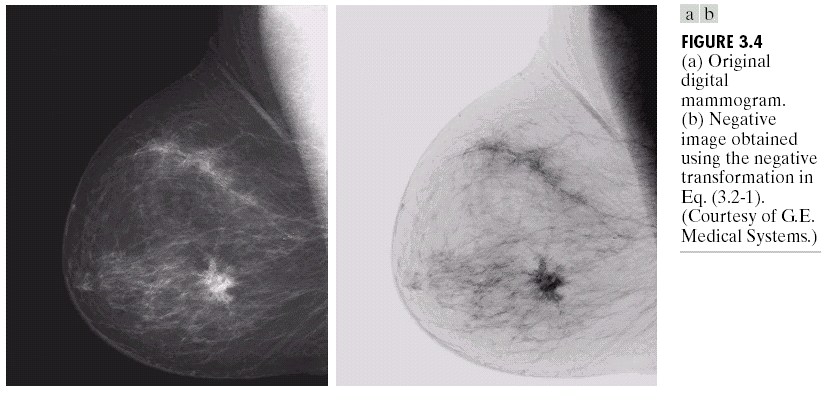
\includegraphics[width=0.6\linewidth]{fig/trans-inverse.png}
\end{figure}
\item 对数变换:$s=c\log(1+r)$,$c$是常数,$r\geq 0$,适合大范围的数据压缩。
任何具有对数函数曲线形状的变换都可以完成灰度的压缩和扩展功能。 
\begin{figure}[H]
\centering
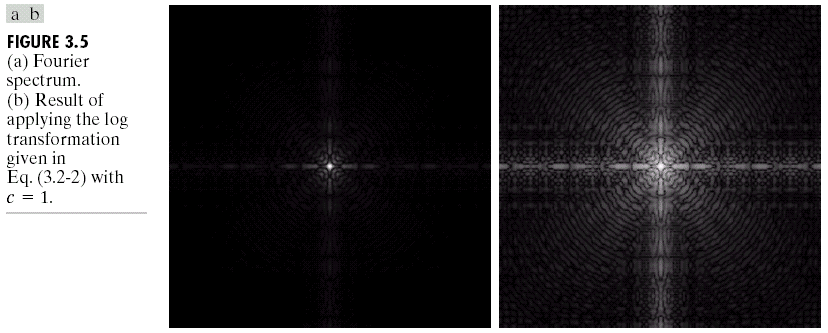
\includegraphics[width=0.6\linewidth]{fig/trans-log.png}
\end{figure}
\item 幂次变换:$s=cr^\gamma$,$c$和$\gamma$都为正常数
\begin{figure}[H]
\centering
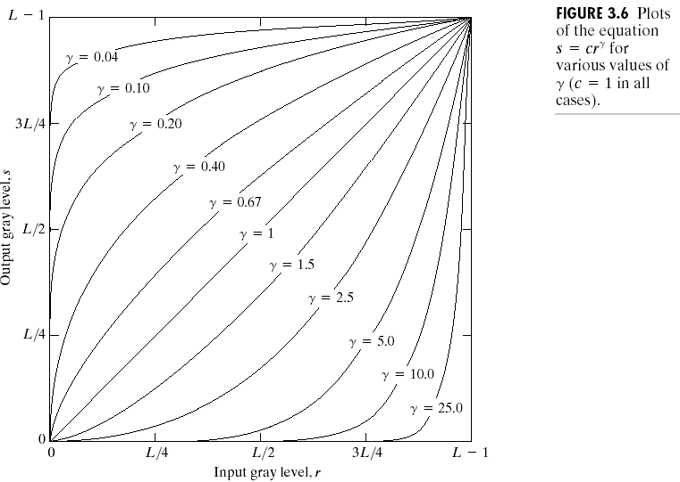
\includegraphics[width=0.6\linewidth]{fig/trans-power.png}
\end{figure}
伽马校正:大量的图像设备如捕捉卡、打印机、数码相机以及显示装置的响应(输出)就对应一个幂函数,通常称这个幂函数的指数为gamma。纠正这个幂次响应的处理称为伽玛校正(gamma correction)。
\begin{figure}[H]
\centering
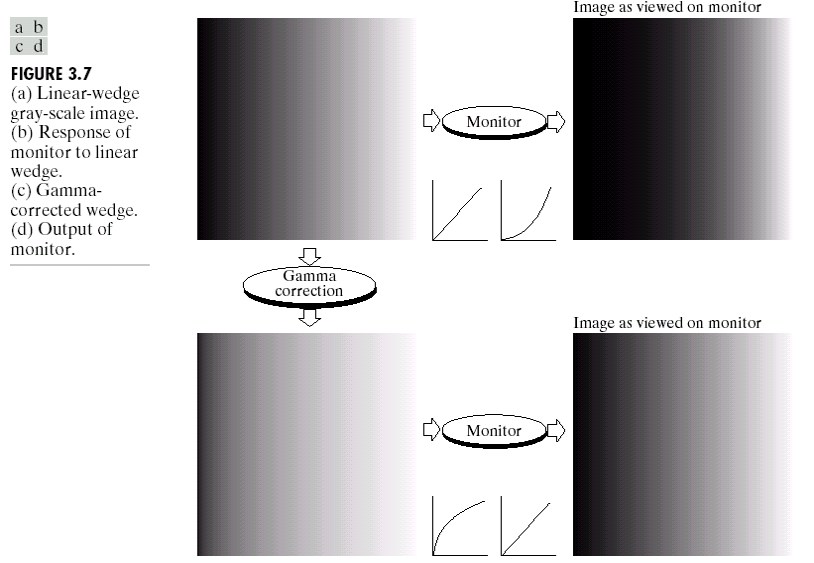
\includegraphics[width=0.6\linewidth]{fig/trans-gamma.png}
\end{figure}
在一般的图像处理软件中,几乎都有伽玛校正的功能。这个功能可用于调整图像的对比度。如果图像偏暗,有些低灰度值的细节被掩盖时,可考虑用指数$\gamma<1$的伽玛校正(变亮);反之,$\gamma>1$的校正对那些被“漂白”的细节会起作用(变暗)。
\item 分段线性变换
\begin{figure}[H]
\centering
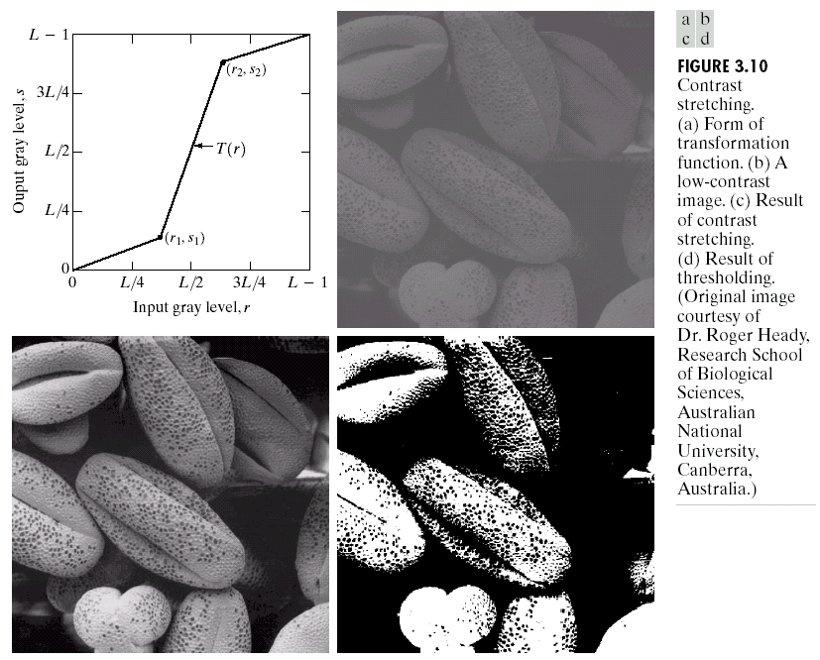
\includegraphics[width=0.6\linewidth]{fig/trans-by-cases.png}
\end{figure}
\item 灰度切割:在图像中提高特定灰度的亮度
\begin{figure}[H]
\centering
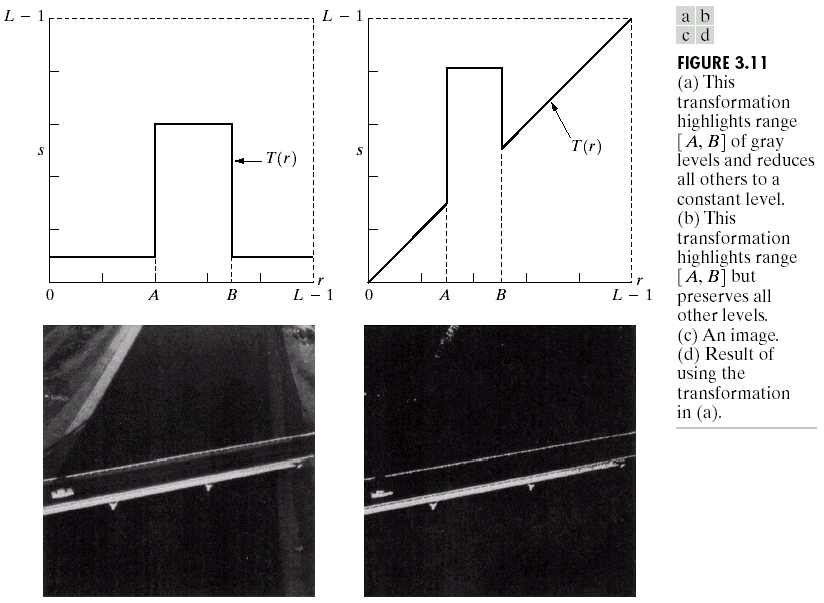
\includegraphics[width=0.6\linewidth]{fig/trans-cut.png}
\end{figure}
\end{itemize}

位图切割:8位灰度图象可以分割成8个位面,每个是一个二值图像(中间切一半)。
\textbf{高位}表示了\textbf{重要的信息},\textbf{低位}给出了\textbf{不同程度的细节}。
\begin{figure}[H]
\centering
\begin{tabular}{cc}
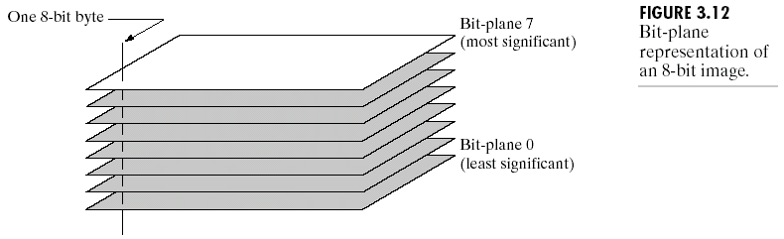
\includegraphics[width=0.5\linewidth]{fig/bitmap.png}&
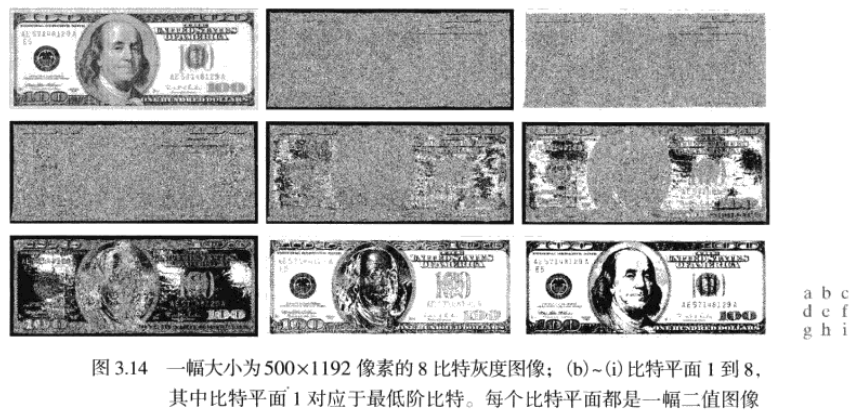
\includegraphics[width=0.5\linewidth]{fig/bitmap-dollars.png}
\end{tabular}
\end{figure}

位图的作用
\begin{itemize}
	\item 信息隐藏:藏在中间位,低位会被丢弃,高位太清楚
	\item 视频传输:先传高位,再传低位,逐渐清晰
\end{itemize}

\subsection{直方图}
\begin{definition}[直方图]
灰度级别为$[0,L-1]$(直方图一定从0开始!)。数字图像直方图是离散函数$h(r_k)=n_k$,其中$r_k$是第$k$级灰度,$n_k$是图像中灰度级为$r_k$的像素个数(频数)。
除以总数$n$就得到归一化的直方图。
\end{definition}

\subsubsection{直方图均衡化}
有亮度差才能看到细节,最好是均衡分布,实现\textbf{高对比度}。
\begin{figure}[H]
\centering
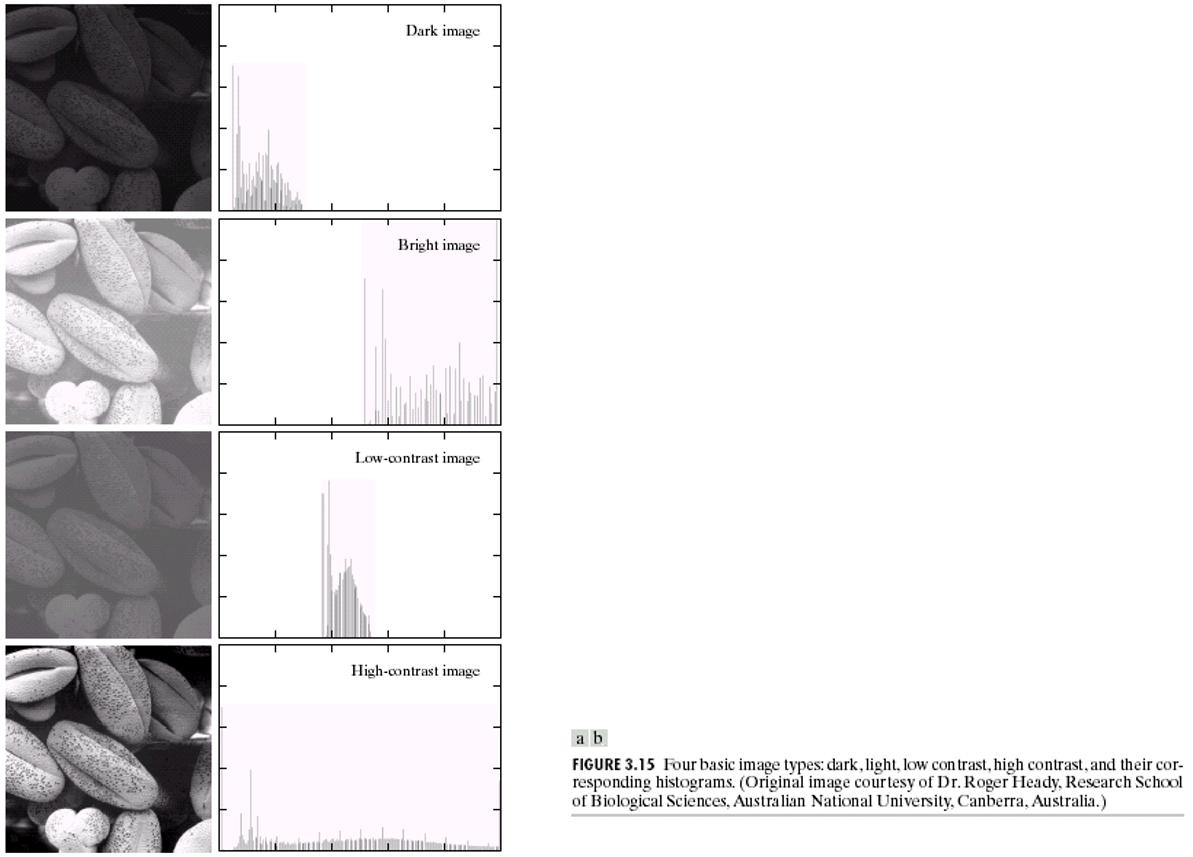
\includegraphics[width=0.6\linewidth]{fig/histogram-quality.png}
\end{figure}

直方图均衡化/线性化则是寻求一种变换使得变换后的图像具有尽可能均匀分布的直方图,用于图像增强最大的特点是自动化,有强大的适应性强的功能。
通常需要满足下列条件:
\begin{itemize}
	\item $T(r)$在$0\leq r\leq L-1$中为单值且单调递增
	\item 当$0\leq r\leq L-1$时,$0\leq T(r)\leq L-1$
\end{itemize}
步骤如下:
\begin{enumerate}
	\item 概率$p_r(r_k)=n_k/n,k=0,1,2,\ldots,L-1$
	\item 累计分布函数(PDF)
	\[P(r_k)=\sum_{j=0}^k p_r(r_j)=\sum_{j=0}^k\frac{n_j}{n},k=0,1,2,\ldots,L-1\]
	\item 变换函数
	\[s_k=T(r_k)=(L-1)\cdot\sum_{j=0}^k\frac{n_j}{n},k=0,1,2,\ldots,L-1\]
	\item 将$s_k$四舍五入转换为标准灰度级别,如有相同$\lceil s_k\rceil$则合并
\end{enumerate}
\begin{figure}[H]
\centering
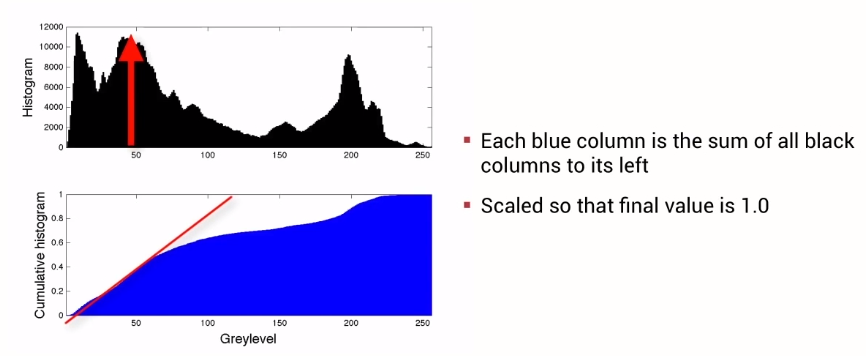
\includegraphics[width=0.8\linewidth]{fig/histogram-normalization.png}
\end{figure}
\begin{analysis}
若$r$为离散型随机变量,$T(r)$为单调递增函数($T^{-1}$存在且单调),且$s=T(r)$,则由概率论有
\[p_s(s)=p_r(r)\pd{r}{s}\Big|_{r=T^{-1}(s)}=p_s(T^{-1}(s))|T^{-1}(s)|\]
考虑变换函数为$r$的累积分布函数(CDF)
\[s=T(r)=\intabu{0}{r}{p_r(\omega)}{\omega}\]
对$s$求导并代入上面的式子可得$p_s(s)=1$,故实现均衡。
算法实际上就是求累积分布函数,使得原本亮度小的像素能够映射到亮度大的空间。
\end{analysis}

\subsubsection{直方图匹配}
当两幅图像比对时,通常要使其直方图形式一致(如不同光照条件下的同一场景)。
先是做空间归一化(伸缩、旋转),然后再做像素的归一化。

做法是使两幅图像均衡化后的结果相同,即
\[\begin{aligned}
s&=T(r)=\intabu{0}{r}{p_r(w)}{w}\\
s&=G(z)=\intabu{0}{z}{p_z(t)}{t}\\
\implies z&=G^{-1}(s)=G^{-1}(T(r))
\end{aligned}\]

具体步骤如下:
\begin{enumerate}
	\item 计算出原图的直方图
	\[s_k=T(r_k)=(L-1)\sum_{j=0}^k\frac{n_j}{n}\]
	\item 给出输出图像期望的直方图$p_z(z)$,并令
	\[v_k=G(z_k)=(L-1)\sum_{i=0}^kp_z(z_i)=s_k\]
	\item 寻找区间$[0,L-1]$的最小整数$\hat{z}$,使得
	\[G(\hat{z})-s_k\geq 0\]
	即由$k$映射到$\hat{z}$
\end{enumerate}

\begin{definition}[$n$阶矩]
设$p_r(r_k)=n_k/n$,则$r$的第$n$阶中心矩为
\[\mu_r(r_k)=\sum_{i=0}^{L-1}(r_i-\bar{r})^np(r_k)\]
其中$\bar{r}=\sum_{i=1}^{L-1}r_ip(r_i)$为$r$的平均值。
特别地,当$n=2$时为方差。
\end{definition}


\subsection{空间滤波基础}
滤波的概念来自信号处理中的傅里叶变换,空间滤波指的是直接对图像像素进行处理的操作。
滤波器(filter)有时也叫掩模(mask)、核(kernel)、模板(template)或窗口(window)。

\subsubsection{线性滤波}
空间域线性滤波基本公式:
\[g(x,y)=\sum_{s=-a}^a\sum_{t=-b}^b w(s,t)f(x+s,y+t)\]
常见的情况是,$a=b$为奇数,如1、3、5。

\begin{definition}[相关与卷积]
一个$m\times n$的滤波器$w(x,y)$与$M\times N$图像$f(x,y)$的相关操作定义为
\[w(x,y)\circ f(x,y)=\sum_{s=-a}^a\sum_{t=-b}^b w(s,t)f(x+s,y+t)\]
一个$m\times n$的滤波器$w(x,y)$与$M\times N$图像$f(x,y)$的卷积定义为
\[w(x,y)*f(x,y)=\sum_{s=-a}^a\sum_{t=-b}^b w(s,t)f(x-s,y-t)\]
其中右侧等号表示将$f$旋转$180\degree$(或先沿$x$轴翻折,再沿$y$轴翻折)
\end{definition}
\begin{figure}[H]
\centering
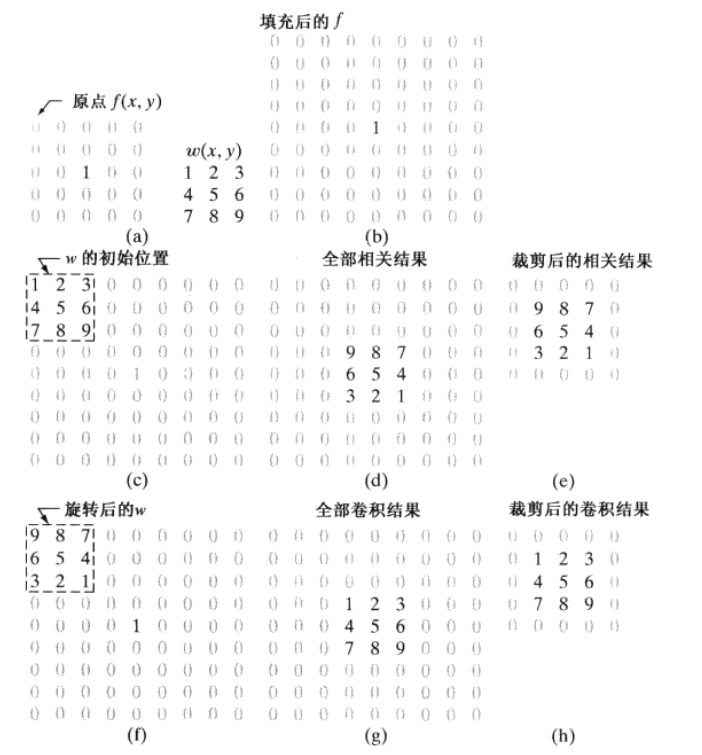
\includegraphics[width=0.5\linewidth]{fig/convolution_and_correlation.png}
\end{figure}

空间滤波对边界的处理方法
\begin{itemize}
	\item 重复边缘值
	\item 卷绕输入图像
	\item 补零(最常用)
	\item 勿略
\end{itemize}

常用的平滑滤波器(左侧是均值滤波)
\[g(x,y)=\frac{\disp\sum_{s=-a}^a\sum_{t=-b}^b w(s,t)f(x+s,y+t)}{\disp\sum_{s=-a}^a\sum_{t=-b}^b w(s,t)}\]
\begin{center}
\begin{tabular}{|c|c|c||c|c|c|}\hline
1/9 & 1/9 & 1/9 & 1/16 & 1/8 & 1/16\\\hline
1/9 & 1/9 & 1/9 & 1/8 & 1/4 & 1/8 \\\hline
1/9 & 1/9 & 1/9 & 1/16 & 1/8 & 1/16\\\hline
\end{tabular}
\end{center}

\subsubsection{非线性滤波}
排序统计滤波器是一种非线性的、 非卷积滤波器。
排序统计滤波器在滤波器包围的像素范围内排序,然后由统计排序结果决定的值代替中心像素的值。
按排序输出的位置分,可分为:中值滤波、最大值滤波、最小值滤波。

中值滤波比均值滤波更适合做\textbf{椒盐噪声}\footnote{特别大或特别小的噪声}的去除,因为噪声总是最大最小,故做中值滤波容易去除。
\begin{figure}[H]
\centering
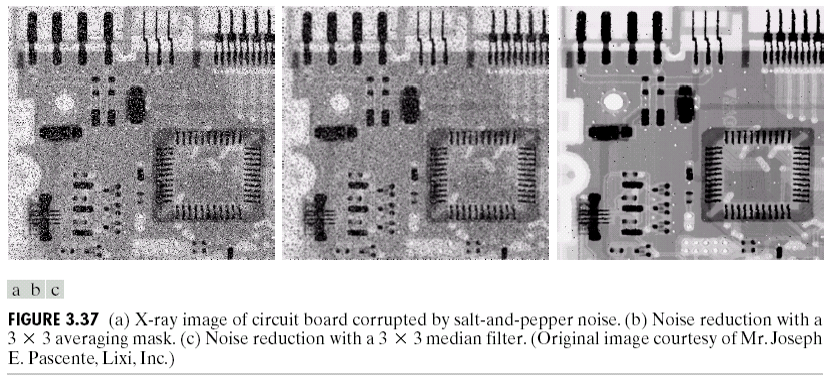
\includegraphics[width=0.8\linewidth]{fig/salt-and-pepper-noise.png}
\end{figure}

同理除了中值滤波,也可以构造第$X$百分点的滤波器。
通常$X<50$图像趋于变暗,$X>50$图像趋于变亮。


\subsection{图像锐化}
\subsubsection{图像微分}
\textbf{积分运算可以做平滑,微分运算可以做锐化!}
锐化的目的即突出图像中的细节或者增强被模糊的细节。

考虑离散情况
\[\begin{cases}
\pd{f}{x}&=f(x+1)-f(x)\\
\pdd{f}{x}&=f(x+1)+f(x-1)-2f(x)
\end{cases}\]

斜边缘、$\delta$/冲击边缘、阶梯边缘
\begin{figure}[H]
\centering
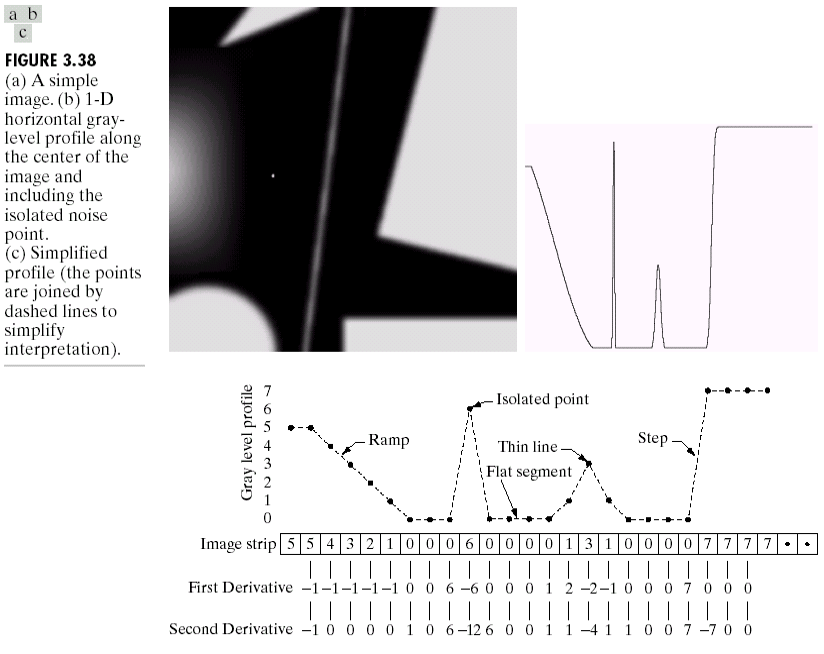
\includegraphics[width=0.6\linewidth]{fig/differential.png}
\end{figure}
\begin{itemize}
\item 一阶微分产生较“宽”的边界,二阶微分产生较“细”的边界
\item 二阶微分处理对细节有较强的响应,如细线和孤立点
\item 一阶微分对阶梯状的灰度变化有较强的响应
\item 二阶微分在处理阶梯状灰度变化时产生双响应
\item 如果灰度的变化相似,二阶微分对线的反应比对阶梯强,对点的反应比对线强
\end{itemize}

\subsubsection{拉普拉斯算子}
\begin{definition}[拉普拉斯(Laplacian)算子]
对连续函数情形,最简单且各向同性的二阶微分算子是拉普拉斯算子
\[\nabla^2 f=\pdd{f}{x}+\pdd{f}{y}\]
离散情况
\[\nabla^2=f(x+1,y)+f(x-1,y)+f(x,y+1)+f(x,y-1)-4f(x,y)\]
\end{definition}
拉普拉斯变换目的是\textbf{获得细节},加回原图像才能进行锐化。
\begin{figure}[H]
\centering
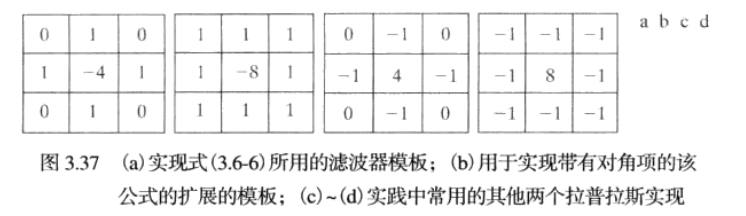
\includegraphics[width=0.6\linewidth]{fig/laplacian_mask.png}
\end{figure}

其实直接从滤波器的表示也可以直观看出这种滤波对图像的突变有比较强的响应(即在突变的位置有较大的输出值),对灰度变化缓慢的区域滤波响应的值会变得很小(变暗)。因此,用拉普拉斯算子作用后,产生的图像将是在暗背景上的一些灰色边线和一些突变点。若将原始图像叠加到拉普拉斯变换后的图像,既可以保护拉普拉斯锐化处理的效果,同时又能复原背景信息。 
拉普拉斯图像增强基本方法:
\[g(x,y)=\begin{cases}
f(x,y)-\nabla^2f & \text{拉普拉斯滤波中心系数为负}\\
f(x,y)+\nabla^2f & \text{拉普拉斯滤波中心系数为正}
\end{cases}\]
\begin{figure}[H]
\centering
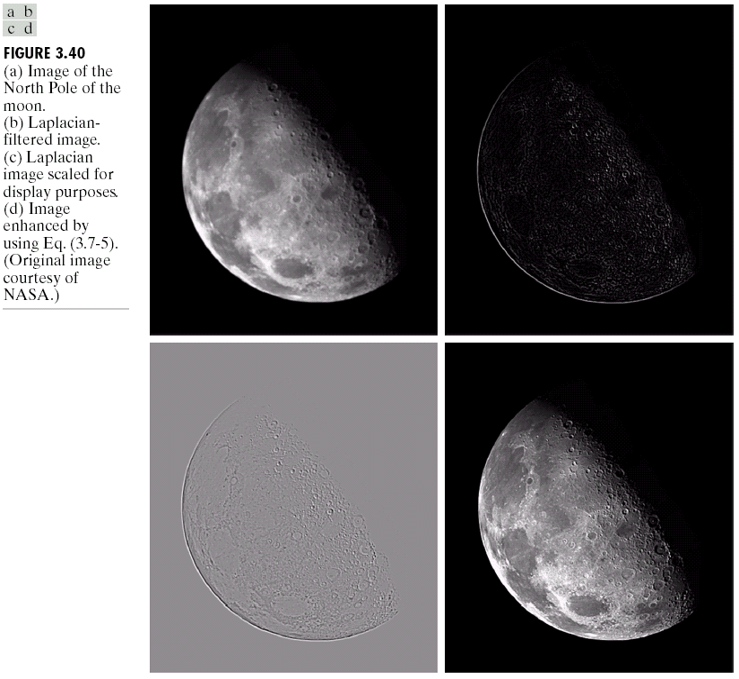
\includegraphics[width=0.6\linewidth]{fig/Laplacian.png}
\end{figure}

\begin{definition}[反锐化掩膜(unsharp masking)]
把原图的一个模糊过的图像从原图中减去,从而得到一个相对清晰的图像
\[f_s(x,y)=f(x,y)-\bar{f}(x,y)\]
就像一个模糊的负片和一个正片放在一起冲洗出相对清晰的照片
\end{definition}
\begin{definition}[高提升滤波(high-boost filtering)]
添加一个系数项$A$得到
\[f_{hb}(x,y)=Af(x,y)-\bar{f}(x,y)=(A-1)f(x,y)+f_s(x,y)\]
其中$A\geq 1$,目的为提升原图亮度,前一部分调整了原图的灰度,后一部分是锐化过的图像。
$A$越大则细节越不清晰,因为原图变亮了。
\end{definition}

可以得到基于拉普拉斯算子的高提升滤波
\[f_{hb}(x,y)=
\begin{cases}
Af(x,y)-\nabla^2 f & \text{Laplacian中心系数为负}\\
Af(x,y)+\nabla^2 f & \text{Laplacian中心系数为正}
\end{cases}\]
当$A=1$时就是拉普拉斯图像增强方法,当$A$足够大时,锐化效果将变得不明显。
\begin{figure}[H]
\centering
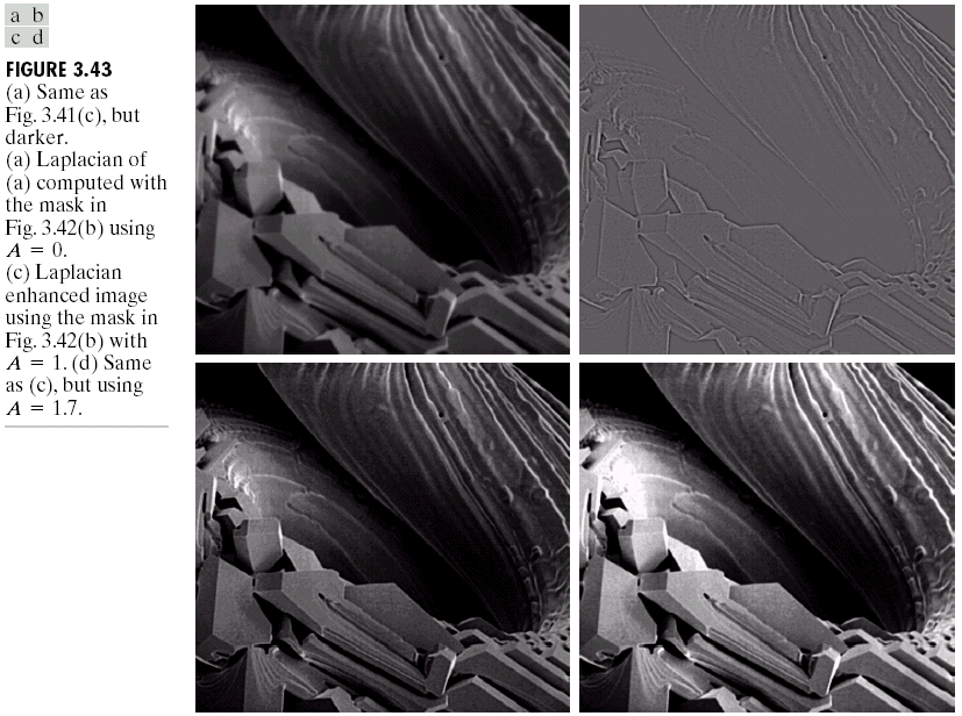
\includegraphics[width=0.6\linewidth]{fig/high-boost.png}
\end{figure}

\subsubsection{梯度}
一阶微分在灰度的跳跃性间断处(边界处)有较强的响应,所以在一些情况下也可以用于图像增强,常用作\textbf{边缘检测}。
考虑二维函数的梯度
\[\nabla f=\bmat{G_x & G_y}=\bmat{\pd{f}{x} & \pd{f}{y}}\]
定义$L_2$范数/模
\[\nabla f=(G_x^2+G_y^2)^{1/2}=\lrp{\lrp{\pd{f}{x}}^2+\lrp{\pd{f}{x}}^2}^{1/2}\]
$L_2$模具有各向同性的性质,但计算不方便,故常用$L_1$范数做代替
\[\nabla f\approx |G_x|+|G_y|\]
注意:通常在不引起混淆的情况下,把梯度的模称为梯度。
\begin{itemize}
\item Robert交叉梯度算子
\[\nabla f=|z_9-z_5|+|z_8-z_6|\]
\item Sobel算子:水平边缘增强
\[\nabla f=|(z_7+2z_8+z_9)-(z_1+2z_2+z_3)|+|(z_3+2z_6+z_9)-(z_1+2z_4+z_7)|\]
\begin{figure}[H]
\centering
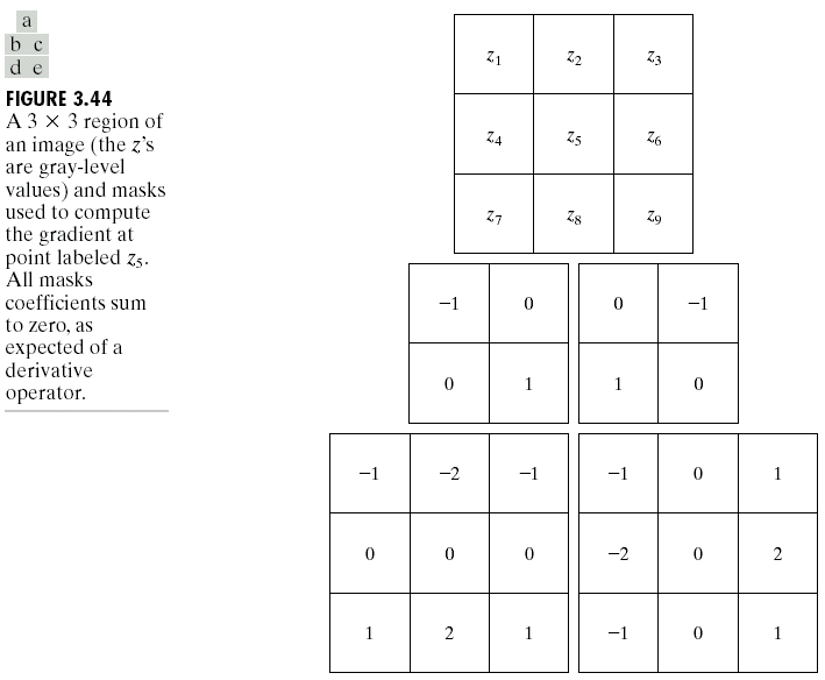
\includegraphics[width=0.4\linewidth]{fig/sobel_and_robert.png}
\end{figure}
\end{itemize}

通常实际使用时是多种滤波器混合使用。
下列为Matlab中预定义的滤波器。
\begin{itemize}
\item Gaussian 低通滤波器
\item Sobel 水平边缘增强滤波器
\item Prewitt 水平边缘增强滤波器:将Sobel的系数绝对值全改为1
\item Laplacian 近似二维拉普拉斯运算滤波器
\item Log (Laplacian of Gaussian)高斯拉普拉斯滤波器
\item Average 均值滤波器
\item Unsharp 模糊对比增强滤波器
\end{itemize}